\documentclass[twoside]{book}

% Packages required by doxygen
\usepackage{fixltx2e}
\usepackage{calc}
\usepackage{doxygen}
\usepackage[export]{adjustbox} % also loads graphicx
\usepackage{graphicx}
\usepackage[utf8]{inputenc}
\usepackage{makeidx}
\usepackage{multicol}
\usepackage{multirow}
\PassOptionsToPackage{warn}{textcomp}
\usepackage{textcomp}
\usepackage[nointegrals]{wasysym}
\usepackage[table]{xcolor}

% NLS support packages
\usepackage[spanish]{babel}
% Font selection
\usepackage[T1]{fontenc}
\usepackage[scaled=.90]{helvet}
\usepackage{courier}
\usepackage{amssymb}
\usepackage{sectsty}
\renewcommand{\familydefault}{\sfdefault}
\allsectionsfont{%
  \fontseries{bc}\selectfont%
  \color{darkgray}%
}
\renewcommand{\DoxyLabelFont}{%
  \fontseries{bc}\selectfont%
  \color{darkgray}%
}
\newcommand{\+}{\discretionary{\mbox{\scriptsize$\hookleftarrow$}}{}{}}

% Page & text layout
\usepackage{geometry}
\geometry{%
  a4paper,%
  top=2.5cm,%
  bottom=2.5cm,%
  left=2.5cm,%
  right=2.5cm%
}
\tolerance=750
\hfuzz=15pt
\hbadness=750
\setlength{\emergencystretch}{15pt}
\setlength{\parindent}{0cm}
\setlength{\parskip}{3ex plus 2ex minus 2ex}
\makeatletter
\renewcommand{\paragraph}{%
  \@startsection{paragraph}{4}{0ex}{-1.0ex}{1.0ex}{%
    \normalfont\normalsize\bfseries\SS@parafont%
  }%
}
\renewcommand{\subparagraph}{%
  \@startsection{subparagraph}{5}{0ex}{-1.0ex}{1.0ex}{%
    \normalfont\normalsize\bfseries\SS@subparafont%
  }%
}
\makeatother

% Headers & footers
\usepackage{fancyhdr}
\pagestyle{fancyplain}
\fancyhead[LE]{\fancyplain{}{\bfseries\thepage}}
\fancyhead[CE]{\fancyplain{}{}}
\fancyhead[RE]{\fancyplain{}{\bfseries\leftmark}}
\fancyhead[LO]{\fancyplain{}{\bfseries\rightmark}}
\fancyhead[CO]{\fancyplain{}{}}
\fancyhead[RO]{\fancyplain{}{\bfseries\thepage}}
\fancyfoot[LE]{\fancyplain{}{}}
\fancyfoot[CE]{\fancyplain{}{}}
\fancyfoot[RE]{\fancyplain{}{\bfseries\scriptsize Generado por Doxygen }}
\fancyfoot[LO]{\fancyplain{}{\bfseries\scriptsize Generado por Doxygen }}
\fancyfoot[CO]{\fancyplain{}{}}
\fancyfoot[RO]{\fancyplain{}{}}
\renewcommand{\footrulewidth}{0.4pt}
\renewcommand{\chaptermark}[1]{%
  \markboth{#1}{}%
}
\renewcommand{\sectionmark}[1]{%
  \markright{\thesection\ #1}%
}

% Indices & bibliography
\usepackage{natbib}
\usepackage[titles]{tocloft}
\setcounter{tocdepth}{3}
\setcounter{secnumdepth}{5}
\makeindex

% Hyperlinks (required, but should be loaded last)
\usepackage{ifpdf}
\ifpdf
  \usepackage[pdftex,pagebackref=true]{hyperref}
\else
  \usepackage[ps2pdf,pagebackref=true]{hyperref}
\fi
\hypersetup{%
  colorlinks=true,%
  linkcolor=blue,%
  citecolor=blue,%
  unicode%
}

% Custom commands
\newcommand{\clearemptydoublepage}{%
  \newpage{\pagestyle{empty}\cleardoublepage}%
}

\usepackage{caption}
\captionsetup{labelsep=space,justification=centering,font={bf},singlelinecheck=off,skip=4pt,position=top}

%===== C O N T E N T S =====

\begin{document}

% Titlepage & ToC
\hypersetup{pageanchor=false,
             bookmarksnumbered=true,
             pdfencoding=unicode
            }
\pagenumbering{alph}
\begin{titlepage}
\vspace*{7cm}
\begin{center}%
{\Large Práctica P\+R\+O2, Circuito de Torneos de Tenis. \\[1ex]\large version 30 mar 2022 }\\
\vspace*{1cm}
{\large Generado por Doxygen 1.8.14}\\
\end{center}
\end{titlepage}
\clearemptydoublepage
\pagenumbering{roman}
\tableofcontents
\clearemptydoublepage
\pagenumbering{arabic}
\hypersetup{pageanchor=true}

%--- Begin generated contents ---
\chapter{Circuito de torneos de tenis}
\label{index}\hypertarget{index}{}Práctica P\+R\+O2 donde se construye un circuito de torneos de tenis... Se introducen las clases {\itshape \mbox{\hyperlink{class_circuito}{Circuito}}}, {\itshape \mbox{\hyperlink{class_torneo}{Torneo}}}, {\itshape \mbox{\hyperlink{class_categoria}{Categoria}}}, {\itshape \mbox{\hyperlink{class_jugador}{Jugador}}}.

Solo se documentan los elementos públicos... 
\chapter{Índice de clases}
\section{Lista de clases}
Lista de las clases, estructuras, uniones e interfaces con una breve descripción\+:\begin{DoxyCompactList}
\item\contentsline{section}{\mbox{\hyperlink{class_categoria}{Categoria}} \\*Representa la \mbox{\hyperlink{class_categoria}{Categoria}} del torneo }{\pageref{class_categoria}}{}
\item\contentsline{section}{\mbox{\hyperlink{class_circuito}{Circuito}} \\*Representa el \mbox{\hyperlink{class_circuito}{Circuito}} de los torneos }{\pageref{class_circuito}}{}
\item\contentsline{section}{\mbox{\hyperlink{class_jugador}{Jugador}} \\*Representa un \mbox{\hyperlink{class_jugador}{Jugador}} }{\pageref{class_jugador}}{}
\item\contentsline{section}{\mbox{\hyperlink{class_torneo}{Torneo}} \\*Representa un \mbox{\hyperlink{class_torneo}{Torneo}} del circuito }{\pageref{class_torneo}}{}
\end{DoxyCompactList}

\chapter{Indice de archivos}
\section{Lista de archivos}
Lista de todos los archivos con descripciones breves\+:\begin{DoxyCompactList}
\item\contentsline{section}{\mbox{\hyperlink{_categoria_8hh}{Categoria.\+hh}} \\*Especificación de la clase \mbox{\hyperlink{class_categoria}{Categoria}} }{\pageref{_categoria_8hh}}{}
\item\contentsline{section}{\mbox{\hyperlink{_circuito_8hh}{Circuito.\+hh}} \\*Especificación de la clase \mbox{\hyperlink{class_circuito}{Circuito}} }{\pageref{_circuito_8hh}}{}
\item\contentsline{section}{\mbox{\hyperlink{_jugador_8hh}{Jugador.\+hh}} \\*Especificación de la clase \mbox{\hyperlink{class_jugador}{Jugador}} }{\pageref{_jugador_8hh}}{}
\item\contentsline{section}{\mbox{\hyperlink{main_8cc}{main.\+cc}} \\*Programa principal para la práctica de P\+R\+O2, {\itshape \mbox{\hyperlink{class_circuito}{Circuito}} de torneos de tenis} }{\pageref{main_8cc}}{}
\item\contentsline{section}{\mbox{\hyperlink{_torneo_8hh}{Torneo.\+hh}} \\*Especificación de la clase \mbox{\hyperlink{class_torneo}{Torneo}} }{\pageref{_torneo_8hh}}{}
\end{DoxyCompactList}

\chapter{Documentación de las clases}
\hypertarget{class_categoria}{}\section{Referencia de la Clase Categoria}
\label{class_categoria}\index{Categoria@{Categoria}}


Representa la \mbox{\hyperlink{class_categoria}{Categoria}} del torneo.  




\subsection{Descripción detallada}
Representa la \mbox{\hyperlink{class_categoria}{Categoria}} del torneo. 

Dispone de blabalbalbala... 

Definición en la línea 16 del archivo Categoria.\+hh.



La documentación para esta clase fue generada a partir del siguiente fichero\+:\begin{DoxyCompactItemize}
\item 
\mbox{\hyperlink{_categoria_8hh}{Categoria.\+hh}}\end{DoxyCompactItemize}

\hypertarget{class_circuito}{}\section{Referencia de la Clase Circuito}
\label{class_circuito}\index{Circuito@{Circuito}}


Representa el \mbox{\hyperlink{class_circuito}{Circuito}} de los torneos.  




\subsection{Descripción detallada}
Representa el \mbox{\hyperlink{class_circuito}{Circuito}} de los torneos. 

Contiene el ranking y la lista de los torneos... 

Definición en la línea 23 del archivo Circuito.\+hh.



La documentación para esta clase fue generada a partir del siguiente fichero\+:\begin{DoxyCompactItemize}
\item 
\mbox{\hyperlink{_circuito_8hh}{Circuito.\+hh}}\end{DoxyCompactItemize}

\hypertarget{class_jugador}{}\section{Referencia de la Clase Jugador}
\label{class_jugador}\index{Jugador@{Jugador}}


Representa un \mbox{\hyperlink{class_jugador}{Jugador}}.  


\subsection*{Métodos públicos}
\begin{DoxyCompactItemize}
\item 
\mbox{\hyperlink{class_jugador_a232c46f75691af6210096e5972535d71}{Jugador}} ()
\begin{DoxyCompactList}\small\item\em Creadora por defecto. \end{DoxyCompactList}\end{DoxyCompactItemize}


\subsection{Descripción detallada}
Representa un \mbox{\hyperlink{class_jugador}{Jugador}}. 

Dispone de blablabla... 

Definición en la línea 14 del archivo Jugador.\+hh.



\subsection{Documentación del constructor y destructor}
\mbox{\Hypertarget{class_jugador_a232c46f75691af6210096e5972535d71}\label{class_jugador_a232c46f75691af6210096e5972535d71}} 
\index{Jugador@{Jugador}!Jugador@{Jugador}}
\index{Jugador@{Jugador}!Jugador@{Jugador}}
\subsubsection{\texorpdfstring{Jugador()}{Jugador()}}
{\footnotesize\ttfamily Jugador\+::\+Jugador (\begin{DoxyParamCaption}{ }\end{DoxyParamCaption})}



Creadora por defecto. 

Se ejecuta automáticamente al declarar un \mbox{\hyperlink{class_jugador}{Jugador}}. \begin{DoxyPrecond}{Precondición}
{\itshape cierto} 
\end{DoxyPrecond}
\begin{DoxyPostcond}{Postcondición}
El resultado es un \mbox{\hyperlink{class_jugador}{Jugador}} sin inicializar 
\end{DoxyPostcond}


La documentación para esta clase fue generada a partir del siguiente fichero\+:\begin{DoxyCompactItemize}
\item 
\mbox{\hyperlink{_jugador_8hh}{Jugador.\+hh}}\end{DoxyCompactItemize}

\hypertarget{class_torneo}{}\section{Referencia de la Clase Torneo}
\label{class_torneo}\index{Torneo@{Torneo}}


Representa un \mbox{\hyperlink{class_torneo}{Torneo}} del circuito.  




\subsection{Descripción detallada}
Representa un \mbox{\hyperlink{class_torneo}{Torneo}} del circuito. 

Contiene los datos de un \mbox{\hyperlink{class_torneo}{Torneo}}... 

Definición en la línea 16 del archivo Torneo.\+hh.



La documentación para esta clase fue generada a partir del siguiente fichero\+:\begin{DoxyCompactItemize}
\item 
\mbox{\hyperlink{_torneo_8hh}{Torneo.\+hh}}\end{DoxyCompactItemize}

\chapter{Documentación de archivos}
\hypertarget{_categoria_8hh}{}\section{Referencia del Archivo Categoria.\+hh}
\label{_categoria_8hh}\index{Categoria.\+hh@{Categoria.\+hh}}


Especificación de la clase \mbox{\hyperlink{class_categoria}{Categoria}}.  


\subsection*{Clases}
\begin{DoxyCompactItemize}
\item 
class \mbox{\hyperlink{class_categoria}{Categoria}}
\begin{DoxyCompactList}\small\item\em Representa la \mbox{\hyperlink{class_categoria}{Categoria}} del torneo. \end{DoxyCompactList}\end{DoxyCompactItemize}


\subsection{Descripción detallada}
Especificación de la clase \mbox{\hyperlink{class_categoria}{Categoria}}. 


\hypertarget{_circuito_8hh}{}\section{Referencia del Archivo Circuito.\+hh}
\label{_circuito_8hh}\index{Circuito.\+hh@{Circuito.\+hh}}


Especificación de la clase \mbox{\hyperlink{class_circuito}{Circuito}}.  


Dependencia gráfica adjunta para Circuito.\+hh\+:\nopagebreak
\begin{figure}[H]
\begin{center}
\leavevmode
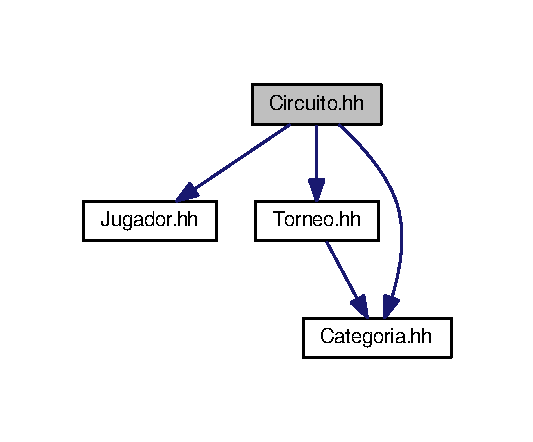
\includegraphics[width=256pt]{_circuito_8hh__incl}
\end{center}
\end{figure}
\subsection*{Clases}
\begin{DoxyCompactItemize}
\item 
class \mbox{\hyperlink{class_circuito}{Circuito}}
\begin{DoxyCompactList}\small\item\em Representa el \mbox{\hyperlink{class_circuito}{Circuito}} de los torneos. \end{DoxyCompactList}\end{DoxyCompactItemize}


\subsection{Descripción detallada}
Especificación de la clase \mbox{\hyperlink{class_circuito}{Circuito}}. 


\hypertarget{_jugador_8hh}{}\section{Referencia del Archivo Jugador.\+hh}
\label{_jugador_8hh}\index{Jugador.\+hh@{Jugador.\+hh}}


Especificación de la clase \mbox{\hyperlink{class_jugador}{Jugador}}.  


\subsection*{Clases}
\begin{DoxyCompactItemize}
\item 
class \mbox{\hyperlink{class_jugador}{Jugador}}
\begin{DoxyCompactList}\small\item\em Representa un \mbox{\hyperlink{class_jugador}{Jugador}}. \end{DoxyCompactList}\end{DoxyCompactItemize}


\subsection{Descripción detallada}
Especificación de la clase \mbox{\hyperlink{class_jugador}{Jugador}}. 


\hypertarget{main_8cc}{}\section{Referencia del Archivo main.\+cc}
\label{main_8cc}\index{main.\+cc@{main.\+cc}}


Programa principal para la práctica de P\+R\+O2, {\itshape \mbox{\hyperlink{class_circuito}{Circuito}} de torneos de tenis}.  


\subsection*{Funciones}
\begin{DoxyCompactItemize}
\item 
int \mbox{\hyperlink{main_8cc_ae66f6b31b5ad750f1fe042a706a4e3d4}{main}} ()
\begin{DoxyCompactList}\small\item\em Programa principal para la práctica de P\+R\+O2, {\itshape \mbox{\hyperlink{class_circuito}{Circuito}} de torneos de tenis}. \end{DoxyCompactList}\end{DoxyCompactItemize}


\subsection{Descripción detallada}
Programa principal para la práctica de P\+R\+O2, {\itshape \mbox{\hyperlink{class_circuito}{Circuito}} de torneos de tenis}. 



\subsection{Documentación de las funciones}
\mbox{\Hypertarget{main_8cc_ae66f6b31b5ad750f1fe042a706a4e3d4}\label{main_8cc_ae66f6b31b5ad750f1fe042a706a4e3d4}} 
\index{main.\+cc@{main.\+cc}!main@{main}}
\index{main@{main}!main.\+cc@{main.\+cc}}
\subsubsection{\texorpdfstring{main()}{main()}}
{\footnotesize\ttfamily int main (\begin{DoxyParamCaption}{ }\end{DoxyParamCaption})}



Programa principal para la práctica de P\+R\+O2, {\itshape \mbox{\hyperlink{class_circuito}{Circuito}} de torneos de tenis}. 



Definición en la línea 22 del archivo main.\+cc.


\begin{DoxyCode}
22            \{
23 
24   \textcolor{comment}{// Clases: Jugador, Torneo, Categoria, -CIRCUITO-}
25   \mbox{\hyperlink{class_circuito}{Circuito}} Circ;
26   \mbox{\hyperlink{class_torneo}{Torneo}} t;
27   \mbox{\hyperlink{class_categoria}{Categoria}} c;
28   \mbox{\hyperlink{class_jugador}{Jugador}} p;
29 
30   \textcolor{keywordtype}{string} opc; cin >> opc;
31   \textcolor{keywordflow}{while} (opc != \textcolor{stringliteral}{"fin"}) \{
32     \textcolor{keywordflow}{if} (opc == \textcolor{stringliteral}{"nuevo\_jugador"} or opc == \textcolor{stringliteral}{"nj"}) \{
33 
34     \}
35 
36     \textcolor{keywordflow}{else} \textcolor{keywordflow}{if} (opc == \textcolor{stringliteral}{"nuevo\_torneo"} or opc == \textcolor{stringliteral}{"nt"}) \{
37 
38     \}
39 
40     \textcolor{keywordflow}{else} \textcolor{keywordflow}{if} (opc == \textcolor{stringliteral}{"baja\_jugador"} or opc == \textcolor{stringliteral}{"bj"}) \{
41 
42     \}
43 
44     \textcolor{keywordflow}{else} \textcolor{keywordflow}{if} (opc == \textcolor{stringliteral}{"baja\_torneo"} or opc == \textcolor{stringliteral}{"bt"}) \{
45 
46     \}
47 
48     \textcolor{keywordflow}{else} \textcolor{keywordflow}{if} (opc == \textcolor{stringliteral}{"iniciar\_torneo"} or opc == \textcolor{stringliteral}{"it"}) \{
49 
50     \}
51 
52     \textcolor{keywordflow}{else} \textcolor{keywordflow}{if} (opc == \textcolor{stringliteral}{"finalizar\_torneo"} or opc == \textcolor{stringliteral}{"ft"}) \{
53 
54     \}
55 
56     \textcolor{keywordflow}{else} \textcolor{keywordflow}{if} (opc == \textcolor{stringliteral}{"listar\_ranking"} or opc == \textcolor{stringliteral}{"lr"}) \{
57 
58     \}
59 
60     \textcolor{keywordflow}{else} \textcolor{keywordflow}{if} (opc == \textcolor{stringliteral}{"listar\_jugadores"} or opc == \textcolor{stringliteral}{"lj"}) \{
61 
62     \}
63 
64     \textcolor{keywordflow}{else} \textcolor{keywordflow}{if} (opc == \textcolor{stringliteral}{"listar\_torneos"} or opc == \textcolor{stringliteral}{"lt"}) \{
65 
66     \}
67 
68     \textcolor{keywordflow}{else} \textcolor{keywordflow}{if} (opc == \textcolor{stringliteral}{"listar\_categorias"} or opc == \textcolor{stringliteral}{"lc"}) \{
69 
70     \}
71 
72     cin >> opc;
73   \}
74 \}
\end{DoxyCode}

\hypertarget{_torneo_8hh}{}\section{Referencia del Archivo Torneo.\+hh}
\label{_torneo_8hh}\index{Torneo.\+hh@{Torneo.\+hh}}


Especificación de la clase \mbox{\hyperlink{class_torneo}{Torneo}}.  


Dependencia gráfica adjunta para Torneo.\+hh\+:\nopagebreak
\begin{figure}[H]
\begin{center}
\leavevmode
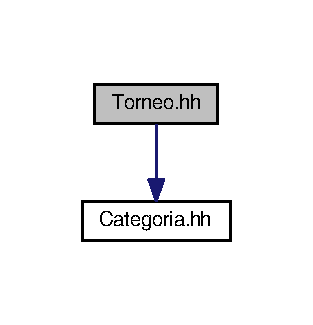
\includegraphics[width=150pt]{_torneo_8hh__incl}
\end{center}
\end{figure}
\subsection*{Clases}
\begin{DoxyCompactItemize}
\item 
class \mbox{\hyperlink{class_torneo}{Torneo}}
\begin{DoxyCompactList}\small\item\em Representa un \mbox{\hyperlink{class_torneo}{Torneo}} del circuito. \end{DoxyCompactList}\end{DoxyCompactItemize}


\subsection{Descripción detallada}
Especificación de la clase \mbox{\hyperlink{class_torneo}{Torneo}}. 


%--- End generated contents ---

% Index
\backmatter
\newpage
\phantomsection
\clearemptydoublepage
\addcontentsline{toc}{chapter}{Índice}
\printindex

\end{document}
